\documentclass[a4paper,preprint]{sig-alternate}

\usepackage{times}
\usepackage{helvet}
\usepackage{courier}
\usepackage{microtype}
\usepackage{hyperref}

\frenchspacing

\toappear{}

\usepackage{blindtext}

\begin{document}

\title{Robustness \& Graph (Convolutional) Neural Networks}

\numberofauthors{1}
%
\author{
%
\alignauthor Tim Bohne\\
\email{tbohne@uni-osnabrueck.de}
}

\maketitle

% TODO: Gliederung für das Paper überlegen / Referenzen / stichpunktartig Inhalte andeuten

\begin{abstract}
\begin{quote}
TBD
\end{quote}
\end{abstract}

\section{Introduction}

The intent of this paper is to provide a brief overview of the current state of research in the domain of
robust graph (convolutional) neural networks. The focus is on the robustness of these models. Since they have proven to be quite successful in
various practical applications, it is quite obvious that the robustness of such models is of relevance.
After giving some motivation and introduction into GNNs and particularly GCNs and their possible practical applications,
an overview of the current results is presented. Finally, there will be some notes on possible future research that is still open.\newline

\section{Background}

A currently very active research area inside the field of machine learning or more precisely deep learning considers models to learn
from graph inputs. Those models are called graph neural networks (GNNs). Graphs are useful data structures in complex real-life
applications such as modeling physical systems, learning molecular fingerprints, controlling traffic networks, and recommending 
friends in social networks.\cite{article}
Therefore, it is reasonable to think about combining graphs as data structure with state-of-the art machine learning models.
However, these tasks require dealing with non-Euclidean graph data that contains rich relational information betwenn elements and
cannot be well handled by traditional deep learning models which usually work with data represented in the Eculidean domain, e.g. in the
fields of computer vision (images) or natural language processing (text).\cite{article}\newline
There are numerous reports of convincing performance of GNNs in practical applications (e.g. (add sources))
especially in the task of semi-supervised node classificaton.\cite{xu2019topology}
Further typical applications for graphs as non-Euclidean data structure in machine learning are link prediction and clustering.\cite{zhou2019graph}\newline
In summary, GNNs are models to conduct deep learning with graph data.\newline

\subsection{Motivation}

One of the most important types of models that contributed to the great success of deep learning are convolutional neural networks (CNNs).
GNNs are motivated by CNNs which are capable of extracting and composing multi-scale localized spatial features
for features of high representation power, but can only operate on Euclidean data like images and text.\cite{article}
Thus, the idea is to generalize CNNs to graphs.\newline

The other motivation comes from graph embedding, which learns to represent graph nodes, edges, or subgraphs in low-dimensional vectors.\cite{article}
The authors also highlight that traditional machine learning approaches for graph analysis relied on hand-engineered features and were limited their
inflexibility and high costs.\newline

\subsection{Graph Neural Networks}

In this section, the basic graph neural network model proposed by Scarselli et al. \cite{4700287} gets introduced
based on the description in \cite{article}.\newline

The goal of a GNN is to learn a state embedding $h_v \in \mathbb{R}^S$ for each node that is used to produce an 
output $o_v$, e.g. the distribution of the predicted node label.
The original GNN model works with an undirected homogeneous graph where each node $v$ in the graph has its input features $x_v$
as well as a set of edges $co[v]$ and neighbors $ne[v]$.\newline
The authors illustrate the structure with the example in figure \ref{fig:graph}.
$x_{1}$ is the input feature of $l_1$. $co[l_1]$ contains edges $l_{(1, 4)}, l_{(1, 6)}, l_{(1, 2)}$, and $l_{(3, 1)}$. $ne[l_1]$ contains nodes $l_2, l_3,
l_4,$ and $l_6$.

\begin{figure}[h]
    \centering
    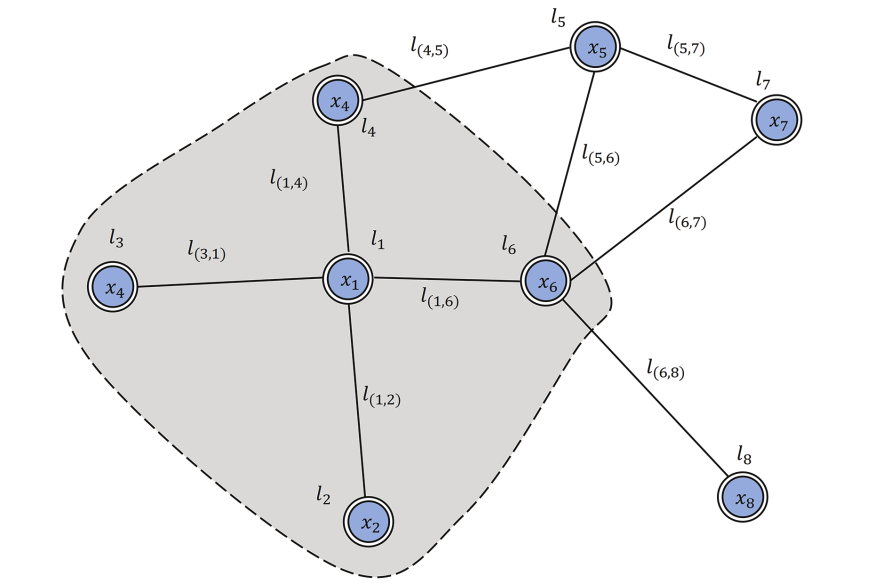
\includegraphics[width=0.4\textwidth]{img/graph.png}
    \caption{\textsc{Graph} \cite{goodfellow2015explaining}.}
    \label{fig:graph}
\end{figure}

There are two important functions, $f$ updates the node state based on the input neighborhood and $g$ computes the output of a node.\newline
Let $x$ be the input feature and $h$ the hidden state:
\begin{itemize}
    \item node embedding: $h_v = f(x_v, x_{co[v]}, h_{ne[v]}, x_{ne[v]})$
    \item output embedding: $o_v = g(h_v, x_v)$
\end{itemize}

Usually, $h_v$ and $o_v$ are described in a more compact form as matrices of stacked states,
outputs, and features:
\begin{itemize}
    \item $H = F(H, X)$
    \item $O = G(H, X_N)$
\end{itemize}
$F$ and $G$ are the stacked versions of $f$ and $g$.\newline

The $t$-th iteration of $H$ is described as $H^{t + 1} = F(H^t, X)$.
With the target information $t_v$ for node $v$, the loss can be written as:
$loss = \sum_{i=1}^p (t_i - o)$
where $p$ is the number of supervised nodes. The learning algorithm is based on a gradient-descent strategy.\newline

The basic GNN model provides a first step towards incorporating neural networks
into the graph domain, but has several limitations \cite{article} which are tackled in various variants
of GNN such as graph convolutional networks (GCNs).\newline

\subsection{Robustness}

Besides the often demonstrated good performance, there is one big issue which is subject to a rather new branch of research inside the field of GNNs 
which is the robustness of such models. There are several publications that analyze the robustness of GNNs to adversarial examples ()
and recently there came up first approaches to strengthen the robustness () or even to certify robustness w.r.t. a certain perturbation set.\newline

Recent advancements in deep neural networks for graph-structured data have led to state-of-the-art performance on recommender system benchmarks.\cite{Ying_2018}
The authors describe a large-scale deep recommendation engine that they developed and deployed at a major tech company.
The GCN algorithm is trained on $7.5$ billion examples on a graph with $3$ billion nodes and $18$ billion edges.
This example illustrates the need for robust GNNs. Although these systems may be relatively rare in practical applications, especially at
that scale, at the moment, their performance suggests that they will be soon. However, to be able to use such models in good conscience 
in practical applications clearly requires a certain level of robustness.\newline
The vulnerability to adversarial attacks has raised increasing concerns for applying GNNs in safety-critical applications. \cite{jin2020graph}\newline
In the following chapters, we will discuss several approaches to analyze and strengthen the robustness of GNNs.\newline

\textbf{The Problem with Adversarial Perturbations}\newline

A well-studied problem of machine learning models in general is the sensitivity to adversarial perturbations.\cite{goodfellow2015explaining}
The idea of such perturbations which is visualized in fig. \ref{fig:adversarial_example} is that slight changes to the input data
cause an entirely different output of the model and therefore often misclassification.\newline

\begin{figure}[h]
    \centering
    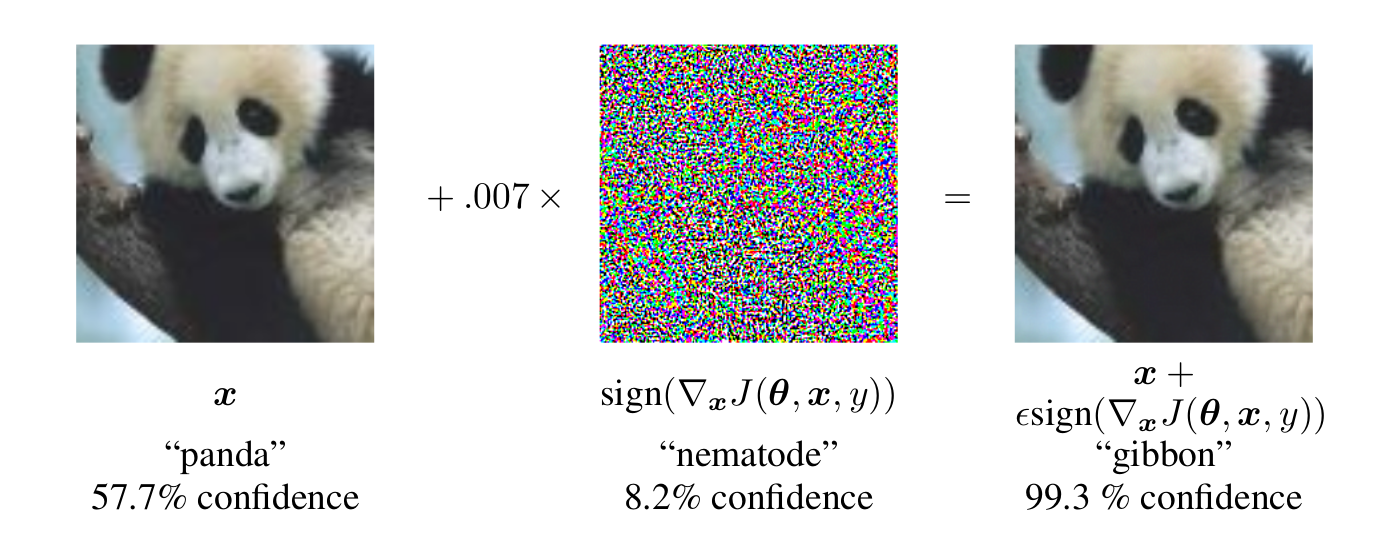
\includegraphics[width=0.5\textwidth]{img/adversarial_example.png}
    \caption{\textsc{Demonstration of fast adversarial example} \cite{goodfellow2015explaining}.}
    \label{fig:adversarial_example}
\end{figure}

Goodfellow et al. \cite{goodfellow2015explaining} face that problem by adversarial training which means that they include adversarially 
perturbed examples into the training procedure to strengthen the robustness of the models. They also introduced fast methods for generating 
those adversarial examples.\newline

Adversarial perturbations are not only a problem for 'classical' machine learning models, but also for GNNs.
Recent works show that graph neural networks are highly non-robust with respect to adversarial attacks on both the graph
structure and the node attributes, making their outcomes unreliable.\cite{Z_gner_2019}\newline
Similarly to the example in fig. \ref{fig:adversarial_example}, small perturbations on the graph structure and node features lead to 
misclassification of the target as depicted in fig. \ref{fig:adversarial_GNN}.\newline

\begin{figure}[h]
    \centering
    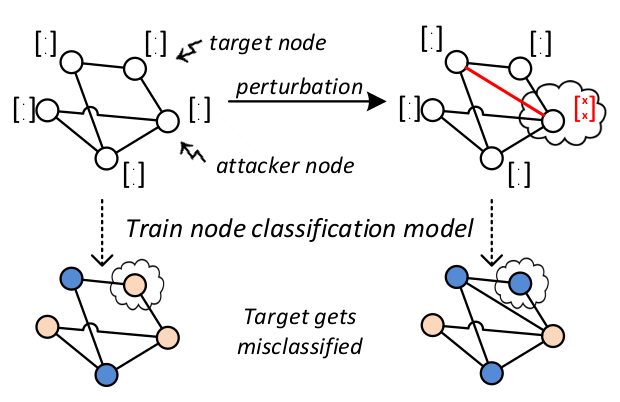
\includegraphics[width=0.4\textwidth]{img/adversarial_GNN.png}
    \caption{\textsc{Demonstration of fast adversarial example} \cite{Z_gner_2019}.}
    \label{fig:adversarial_GNN}
\end{figure}

\section{Literature Review}

This section will provide an overview of the current state of research in the domain of robust GNNs.\newline

Dai et al. \cite{dai2018adversarial} focus on adversarial attacks on graph structured data that fool the model by modifying the
combinatorial structure of the data. They use synthetic and real-world data to show that a family of GNN models are vulnerable
to these attacks, in both the graph-level and node-level classification tasks.\newline
Another approach for adversarial attacks on graph structured data is proposed by Zügner et al. \cite{Z_gner_2018} who focus on node classification
via graph convolutional networks.
They claim that especially in domains where GNNs are used, e.g. the web, adversaries are common and that it is therefore important
to investigate the robustness of such models. They study adversarial attacks on attributed graphs and distinguish between
adversarial attacks on the node's featueres and the graph structure. Their results suggest that the accuracy of node classification
significantly drops even for only a few perturbations which clearly motivates reflections on the robustness of such models, especially
when considering the practical applications.\newline
So far, we talked about adversarial attacks as a quite vague concept. Zügner et al. \cite{zuegner2019adversarial}
introduce them as small deliberate perturbations of data samples in order to achieve the outcome desired by the attacker.
They propose three categories to be considered in the attack model. Those categories are discussed in detail in section \ref{}.
The categories allow more precise considerations of a model's weaknesses and robustness and are later used to compare and interpret results of 
different approaches. Furthermore, they confirm previous claims that small graph perturbations consistently lead to a strong decrease 
in performance for GCNs.\newline

Since the fact that GNNs are vulnerable to adversarial perturbations was confirmed by many publications, the next natural question to ask
is how to defend them against such attacks. 
Direct extension of defense algorithms for classical neural networks based on adversarial samples meets with immediate challenge because
computing the adversarial network costs substantially. \cite{Jin2020} The authors propose to address this issue by perturbing the latent 
representations in GCNs, which not only dispenses with generating adversarial networks, but also attains improved robustness and accuracy 
by respecting the latent manifold of the data. They apply their framework of latent adversarial training on graphs to node classification,
link prediction, and recommender systems and are able to confirm superior robustness in experiments.
When considering the robustness of GNNs, it is of course quite important to have efficient and effective attack methods to test with.
Xu et al. \cite{xu2019topology} present a gradient-based attack method that facilitates the difficulty of tackling discrete graph data
and leads to a noticeable decrease in classification performance. Furthermore, they propose an optimization-based adversarial training
for GNNs which yields higher robustness without sacrificing classification accuracy.\newline
Zhu et al. \cite{10.1145/3292500.3330851} propose Robust GCN (RGCN), a novel model that fortifies GCNs against adversarial attacks.
Instead of representing  nodes as vectors, they adopt Gaussian distributions as the hidden representations of nodes in each
convolutional layer which allows the model to automatically absorb the effects of adversarial changes in the variances of the Gaussian distributions.
Moreover, to remedy the propagation of adversarial attacks in GCNs, they propose a variance-based attention mechanism, i.e. assigning different
weights to node neighborhoods according to their variances when performing convolutions. Their experimental evaluation suggests that
the method can effectively improve the robustness of GCNs.\newline
Another approach to enhance the robustness of GCNs is proposed by Chen et al. \cite{Chen2020} and is based on the idea that
edge manipulations play a key role in graph adversarial attacks. They design a biased graph-sampling scheme to drop graph connections
such that random, sparse and deformed subgraphs are constructed for training and inference thereby alleviating the sensitivity 
to edge manipulations, and thus enhancing the robustness of the models. Their experimental results validate the effectiveness 
against adversarial attacks.\newline
The idea, the approach of Jin et al \cite{jin2020graph} is based on is to defend adversarial attacks by cleaning up the perturbed graph.
The authors state that real-world graphs share some intrinsic properties as they are often low-rank, sparse, and the features of two adjacent
nodes tend to be similar and that adversarial attacks are likely to violate these properties.\newline
They propose the framework Pro-GNN, which can jointly learn a structural graph and a robust GNN model from the perturbed graph guided by
these properties. They are able to show that the proposed framework achieves significantly better performance compared with the state-of-the-art 
defense methods.\newline
Finally, Wang et al. \cite{wang2019graphdefense} propose with GraphDefense a defense algorithm to improve the robustness of GCNs
against adversarial attacks on graph structures and they also discuss what characteristics of defense methods are crucial to improve 
the robustness.\newline

When considering safety-critical applications, it is not only required to be able to defend the system in some scenarios, but there
have to be guarantees about the safety of the system.\newline
Bojchevski et al. \cite{bojchevski2019certifiable} present a first method for verifying certifiable
(non-)robustness to perturbations of the graph structure for a general class of models including GNNs. Additionally, they investigate robust 
training procedures that increase the number of certifiably robust nodes while maintaining or even improving the predictive accuracy.
Their work is limited to a specific class of graph models based on PageRank, not covering the highly important principle of graph convolutional
networks. \cite{10.1145/3394486.3403217}\newline
In \cite{Z_gner_2019}, Zügner et al. propose a first method for certifiable (non-)robustness of GCNs with respect to 
perturbations of the node attributes. If a node has been certified with their method, it is guaranteed to be robust under any
possible perturbation given the attack model. Likewise, they can certify non-robustness and propose a robust semi-supervised training
procedure which improves the robustness with only minimal effect on the predictive accuracy.\newline
Recently, Zügner et al. \cite{10.1145/3394486.3403217} tackle the problem of GCNs under perturbation of the graph structure and propose a method
for certifying their robustness. They show how the problem can be expressed as a well-studied jointly constrained bilinear program and
propose a branch-and-bound algorithm to obtain lower bounds on the global optimum. They decompose the problem into sub-problems that can
be formulated as linear programs and therefore be solved using highly optimized LP-solvers (e.g. CPLEX).\newline

\textbf{Summary}\newline

One could divide the research in the field of robust GNNs roughly into three important phases.
The first phase was to show that GNNs are indeed vulnerable to adversarial perturbations of the graph structure and the node attributes.
Afterwards, in the second phase, several publicatons introduced defense mechanisms against such attacks or novel training procedures 
to strenghten the robustness of the models in some scenarios. Only recently, the third phase began in which first approaches appeared
that are able to not only provide mitigations to adversarial attacks in some scenarios, but to give provable guarantees about the (non-)robustness 
of a model which is key to use them in safety-critical applications in the real world. Because of the relevance of the last phase which 
is an important step in the process of bringing the convincing GNN models into the real world, the main focus of the following chapters
will be on publications from that phase.

\section{Attack Model}

TODO: Not yet sure where to put....

\begin{enumerate}
    \item \textbf{Attacker's goal:} increase the misclassification rate of a node classification algorithm
    \item \textbf{Attacker's knowledge about training data:} input graph, learning model, trained model parameters
    \item \textbf{Attacker's capability:} adversarial attacks should be unnoticed 
\end{enumerate}

\section{Methods}

\pagebreak

\section{Conclusion + Discussion}
TBD

\pagebreak

\bibliographystyle{acm}
\bibliography{bibliography}


\end{document}